\documentclass{report}

\usepackage{fullpage}
\usepackage{verbatim, moreverb, fancybox, framed}
\usepackage{listings, tikz, color, textcomp}
\usepackage{xcolor}
%\usepackage{bera} %attempt at getting a different font
\usepackage[titletoc, title]{appendix}
\usepackage{url, pdfpages, caption}
\usepackage{hyperref}
\usepackage[all]{hypcap}    %for going to the top of an image when a figure reference is clicked -- didn't work for this doc since i'm using minipage instead of the figure environment.

% creates an environment for pre-chapter quotations from famous wise folks
\makeatletter
\renewcommand{\@chapapp}{}% Not necessary...
\newenvironment{chapquote}[2][2em]
  {\setlength{\@tempdima}{#1}%
   \def\chapquote@author{#2}%
   \parshape 1 \@tempdima \dimexpr\textwidth-2\@tempdima\relax%
   \itshape}
  {\par\normalfont\hfill--\ \chapquote@author\hspace*{\@tempdima}\par\bigskip}
\makeatother

% my own colors
\definecolor{codebgcolor}{gray}{0.95}

	%dark scheme
	\definecolor{green}{RGB}{0, 195, 34}
	\definecolor{blue}{RGB}{3,137,156}
	\definecolor{red}{RGB}{255,19,0}
	\definecolor{orange}{RGB}{255,122,0}

	%light scheme
	\definecolor{lgreen}{RGB}{100, 223, 133}
	\definecolor{lblue}{RGB}{99, 173, 208}
	\definecolor{lred}{RGB}{255, 131, 115}
	\definecolor{lorange}{RGB}{255, 190, 115}
	
	%super light scheme
	\definecolor{slgreen}{RGB}{180, 244, 191}
	\definecolor{slblue}{RGB}{178,221,237}
	\definecolor{slred}{RGB}{255,193,188}
	\definecolor{slorange}{RGB}{255,223,188}

\definecolor{keywords}{RGB}{255,0,90}
\definecolor{comments}{RGB}{60,179,113}
\definecolor{fore}{RGB}{249,242,215}
\definecolor{back}{RGB}{51,51,51}
\definecolor{title}{RGB}{255,0,90}

% my own commands
%\newcommand{\new}{\original}
\renewcommand\fbox[1]{\Ovalbox{#1}}	% makin' oval boxes 'round text
\renewcommand*\FrameCommand{\ovalbox}	% makin' oval boxes 'round text (more!)
\newcommand{\dstar}{$\star\star$}	% double star
\newcommand{\ww}{\color{keywords}}	% wayne comments
	% {\ww write comments in this format.}

% configure hyperref, which sets up the internal links
\hypersetup{
	colorlinks=false,
	pdfborder={0 0 0},
	%linkcolor=blue,
	}

%2DO
% this shit still needs work
% configure listing, which does code snippets
\lstset{language=Python,
%	basicstyle=\
	showstringspaces=false,
	lineskip=-2.55pt,
	breakatwhitespace=false,
	morekeywords={self, __init__}
	morestring=[b]",
	upquote=true,
%	stringstyle=\color{title}
%	commentstyle=\color{comments}, 
%	keywordstyle=\color{keywords},
%	backgroundcolor=\color{back}
%	stringstyle=\color{red}
%	showspaces=false,
%    identifierstyle=\color{green},
%    procnamekeys={def,class}
%	tabsize=4
	}

% to link to an external source:
% \href{URL}{text to display}

\renewcommand{\baselinestretch}{2}
\title{FunkyTester Code\\
	\large\emph{Breaking it into Bite-Sized Pieces}}
\author{Montana Goodman}
\begin{document}
\maketitle
\tableofcontents\newpage
%\lstset{language=bash}

%%%%%%%%%%%%%%%%%%%%%%%%%%%%%%%%%%%%%%%%%%%%%%%%%%%%%%%%%%%%%%%%%%%%%%%%%%%%%%%%%%%%%%%%%%%%%%%%%%%%%%%%%%%%%%

% NOTES
% search "REVAMP" for sections that need to be rewritten or reworked or that I'm
% 	generally just not pleased with (or that just needs a second look)
%
% search "REVIEW" for passages that need another look - make sure the grammar is 
%	correct, that the wording is right
%
% search "2DO" for sections that are missing content (partial or entire) and
%	little things that need doing
%	note that a "TODO" search will give results from the text of this manual, which
%		is not ideal
%

% PROJECTS (if there's enough time)
% make a local command for the hyperref parts (customized output)
%
% color directories on different machines(?): see the comment at the bottom of
%	\section{Where Do We Begin?} -- also, background colors for code snippets to
%	change depending on the mahcine they are to be run on
%
% square off the starred areas (these are things i admit to knowing very little to 
%	nothing about
%
% new command for italic text surrounded by double stars
% 
% split appendices up: have each appendix start at a new page
%
% add an "index" type thing at the end with a list of all the pics/screenshots 
%	and links to them in the document
%
% get the internal links to pics set up so that it takes the reader to the top
%	of the pic instead of the bottom
%
% aliases for \texttt{ft}, others (make them \ft?)
%
% get automated Wayne Says... boxes to pop up on the sides: make it an easy command
%	that just does everything fucking perfectly
%

% ****DO THIS****
% Appendices don't need to thread back to the FT code...Appendices can stand on
%	their own. Explain the connections to the code in the meat of the document.
%
% make a yaml appendix (section heartofcode/test)
%
% Make sure every Appendix gets referenced in the document somewhere. otherwise,
%	get rid of the appendix...
%
% Clean up all of the config code (above these notes)
%
% Code snippets: have a key/legend for what the colors mean. green for local
%	machine, blue for testset machine, orange for sshing stuff (where we switch 
%	from one machine to another within the code snippet)
%
% Add GUI screenshots
%

%%%%%%%%%%%%%%%%%%%%%%%%%%%%%%%%%%%%%%%%%%%%%%%%%%%%%%%%%%%%%%%%%%%%%%%%%%%%%%%%%%%%%%%%%%%%%%%%%%%%%%%%%%%%%%
\chapter{First Things First}
\begin{chapquote}{Walt Disney \textit{}}
``The way to get started is to quit talking and begin doing.''
\end{chapquote}

\section{Keep it Zen}
It is important not to get mentally bogged down by all of the code and the seeming lack of structure therein. Reading code is more an exercise in mental perseverance than anything else. The following are a few tips from that may help code comprehension:
	\begin{itemize}
	\item \textbf{Use a debugger}: a debugger allow stepping through the code, seeing where functions are called, who calls them, etc.
	\item \textbf{Take notes}: Taking notes is a valuable tool to help with understanding source code. Notes allow for documentation of areas in the code that are not understood at the time. A developer assigned to the project may be contactedat a leter time for clarification. Keep these notes in a document for future developers to use in their learning process.
	%2DO: make the parenthetical note a sidenote if time
	% Rework entire section
\begin{comment}
	\item \textbf{Don't trust comments}: On the /personal/montana branch (don't understand the lingo? \hyperref[app:git]{\textbf{git it}}), I wrote the majority of the comments and I have a less-than-ideal understanding of programming and Python. If the comments are helpful for you to gain some sort of intuition, then they will have done their job. But if they don't make sense to you or seem more convoluted than the code itself, then by all means go to the code and see for yourself what's going on.
\end{comment}
	\item \textbf{Look at the Code}: To fully understand this document and the software it describes, it is beneficial to have the source code and directory structure available to look at.
	\end{itemize}
Finally, it should be noted that this manual cannot be used to replace time spent reading and understanding the code. This manual is simply a supplement to working through the software and raw code.
%possibly remove final section entirely vvv
\begin{comment}
Finally, I should end with a note about this manual. I am not the expert on this code. I didn't write the code, and it's taken me quite a bit of time to familiarize myself with it. I certainly don't have a complete understanding of every piece of code, but I've done my best to present what I do know and to indicate the portions I am unfamiliar with. When I write about things I don't know much about, I'll surround my conjectures by two stars: \dstar. Hopefully these stars, along with the tone of uncertainty of these passages, will encourage the reader to tread lightly.
\end{comment}
%%%%%%%%%%%%%%%%%%%%%%%%%%%%%%%%%%%%%%%%%
\section{Where to Begin?}
There are a few steps involved in the set up process for the testset software. First, two git repositories must be cloned. One of these contained the source code for the testset -- this is the \texttt{funkytester} directory, minus the contents of its \texttt{ext/emac} subdirectory. The \texttt{ext/emac} subdirectory contains product-specific information and isn't suited for public display on the internet (needed to keep EMAC's clients' information safe). This subdirectory was the second of the repositories we cloned (it contains the \textit{manifest} file, which is very important for running the testset). See \hyperref[sec:gitcloning]{\textbf{Appendix \ref{sec:gitcloning}}} for a detailed walk-through of that process.\\

\begin{comment}
%2DO update the code snippet. talk about server socket whatever.
Getting these repositories installed all of the code we needed in order to run the new testset. Here's how we do that (from the \texttt{funkytester} directory): 
\begin{framed}
	\begin{verbatim}
		$ ./bin/pytest.py -p ext/emac/manifest.yaml
	\end{verbatim}
\end{framed}
Notice that this calls the \texttt{pytest.py} file with that super important manifest file we were just talking about as an argument. I'm not really sure what the \texttt{-p} argument does.
\end{comment}

The next step is to set up for running the testset software via SSH on the testset machine (that is, the physical piece of equipment that actually interfaces with the board). This is important because running the software on a local machine doesn't actually do any testing, it is not connected in any way to a board. Running the software through SSH on the testset machine (this time from the \texttt{projects/funkytester} directory), allows testing of the board hooked to the tester. Go to \hyperref[sec:SSH]{\textbf{Appendix \ref{sec:SSH}}} for more details on that set-up process.
%maybe have different colors for directory names on different machines: explain the colors in the beginning of the document

To run the software, refer to \hyperref[sec:run]{\textbf{Appendix \ref{sec:run}}}.

Finally, open the \texttt{INSTALL} file located in the \texttt{funkytester} directory and install all the necessary software. All of the listed applications are vital to the correct performance of the testset software. If there are still issues running the software after installing everything listed in the \texttt{INSTALL} file, please refer to the suggestions in \hyperref[sec:trouble]{\textbf{Appendix \ref{sec:trouble}}}.

%%%%%%%%%%%%%%%%%%%%%%%%%%%%%%%%%%%%%%%%%
\section{A Bird's Eye View -- Some Insight into the Testset Design and Purpose}
\begin{chapquote}{Linus Torvalds}
``Nobody should start to undertake a large project\ldots And don't expect people to jump in and help you. That's not how these things work.''
\end{chapquote}

%this is good info, but probably not appropriate here. incorporate it into the 
% document as appropriate.
% REVAMP
Before continuing, the README file in the \texttt{funkytester} directory should be read. There is a list of terminology that will be essential to know about when reading through the code. The important thing to keep in mind is that the majority of the items in the terminology list are simply abstractions of real-life objects. For example, the Platform class is an abstraction of the platform. Currently, there are only two platforms -- the GE EVSC Funtional Tester and the Quad Testset. Note that the testset software was designed with the idea that it could be used for any platform that may be developed in the future. That is, there is the potential for the FunkyTester test software to incorporate future testing platforms as well.


%%%%%%%%%%%%%%%%%%%%%%%%%%%%%%%%%%%%%%%%%%%%%%%%%%%%%%%%%%%%%%%%%%%%%%%%%%%%%%%%%%%%%%%%%%%%%%%%%%%%%%%%%%%%%%
\chapter{Looking in Layers} 
\begin{chapquote}{Shrek \textit{}}
``Ogres have layers. Onions have layers. You get it? We both have layers."
\end{chapquote}

% REVIEW
	The architecture of the code can be studied in great detail by looking at each piece of code and it's what code it depends on. Less important is the directory structure that the code is stored in, but it may be helpful to look it briefly. It should be noted however, the directory structure is subject to change without notice. Refactoring the directory structure will not impact the performance of the code, but may cause some temporary confusion.
	
	This document will attempt to give an overview of the general structure of the testset software. Each section in this chapter will take a layer of the structure and overview what each item aims to accomplish. Earlier sections will cover higher level pieces of code while following sections cover deeper sections.
	
\section{Top Level Directory: \texttt{funkytester}}
%REVIEW
Before beginning the discussion on the architecture of the code, it is prudent to look at the root directory of the funkytester software. Typing the \texttt{ls} command while in the \texttt{funkytester} directory will give you the current list of files and subdirectories, an example of which is shown below in \hyperref[fig:top]{\textbf{Figure \ref{fig:top}}}.\\
	
	\begin{minipage}{\linewidth}
		\begin{tikzpicture}
    \node [fill=codebgcolor,rounded corners=5pt]
    {{
        \begin{tabular}{l}
\begin{lstlisting}
/funkytester $ ls
bin/     doc/       ext/      INSTALL  Makefile   pytest_log  resources/  TODO
COPYING  doxy.conf  include/  lib/     py_test.c  README      scripts/
/funkytester $ 

\end{lstlisting}
        \end{tabular}
      }};
  		\end{tikzpicture}
		\captionof{figure}{Layer One: Contents of \texttt{funkytester}}
		\label{fig:top}
	\end{minipage} 
\vspace{5pt}% gives some breathing room below


This section will explain each of the files and directories in turn and give an importance level to each. Most of the files located in this directory are supplemental files, while the directories contain the actual code.

There is at least one file in \texttt{funkytester} that has to do with Doxygen, \texttt{doxy.conf}. Doxygen is software that is used to document the code in a systematic way. The output can be configured by editing the \texttt{doxy.conf} file. \hyperref[app:doxy]{\textbf{Appendix \ref{app:doxy}}} gives more details on the workings of Doxygen, and  shows an example of the commenting style used for it.

\subsection{Peripheral Items}
% README, TODO, COPYING, INSTALL, include, Makefile, py_test.c, pytest_log, 
% RemoteSystemsTempFiles, scripts
These are items of least importance, as far as understanding the FunkyTester code. It is best to just acknowledge that they are there in case they are needed for reference in the future.
\begin{itemize}
	\item \texttt{README}: It should be updated as work progresses, but for now the majority of this file consists of notes for future development. It also describes metadata that is needed for the testset to run. The \hyperref[subsec:medium]{\textbf{next section}} will go more into depth on metadata.
	\item \texttt{TODO}: Detailed list of what needs to be worked on (more specific than \texttt{README}'s visions of the future).
	\item \texttt{COPYING}: Copyright and distribution information.
	\item \texttt{INSTALL}: Gives a list of software required to be installed to run the testset.
	\item \texttt{Makefile}: For use with the make utility. See \hyperref[app:make]{\textbf{Appendix \ref{app:make}}} for more information, but make is not vital for this project.
	%possibly deprecated vvv
	\item \texttt{py\_test.c}: This is a version of the test software written in C?
	\item \texttt{pytest\_log}: Log file that shows exactly what is happening to the code as it executes. Can be viewed live by using the command \texttt{tail -f pytest\_log} while in the funkytester directory.
	\item \texttt{scripts}: At this time there is just one script in this directory. This is an initialization script and is not vital to the understanding of the code.
\end{itemize}


\subsection{Of Medium Importance} \label{subsec:medium}
% ext, resources, doc
% REVIEW
Two of these directories have to do with Platform and Product metadata. The third is the directory containing this manual along with some other helpful items.
\begin{itemize}
	\item \texttt{include/}: Contains the C and C header files used to run most of the tests on the board under test.
	%2DO: more on ext: contains interfaces info for ADAM modules (see the README)
	\item \texttt{ext}: Contains the second repository that had to be cloned when getting set up with the code -- \texttt{emac}. This subdirectory holds data and information about EMAC customers' specific products and cannot be stored publicly.
	\item \texttt{resources}: Contains specifications (manifest files) on EMAC-specific products such as testing platforms.
	\item \texttt{doc}: This directory may not be included with every branch in the repository. If it is included, it will contain this document and the dependancies for this document. Also, in the \texttt{diagrams} subdirectory there are four diagrams that illustrate the hierarchy of the code: a pair for \texttt{funkytester/lib/ft} and a pair for \texttt{funkytester/lib/ui}. Each pair of diagrams consists of a class diagram and a package diagram. These are all .dot format, so xdot may need to be installed in order to view them. It may be helpful to look at these to get an idea of how different parts of \texttt{ft} and \texttt{ui} interact.
\end{itemize}

\subsection{Focus On These Guys}
% bin, lib
The two most important directories in \texttt{funkytester} are \texttt{bin} and \texttt{lib}. The former holds the ``final product": the software we actually run in order to begin testing a board. The latter holds the majority of the rest of the code: the GUI implementation.

\section{Layer Two: Start of the Code} \label{sec:layer2}
After the top layer directory, \texttt{funkytester}, the directory structure does not mean much as far as code architecture is concerned. What is important, however, is the the structure of the classes and functions inside of the file structure.

%\subsection{\texttt{bin}}
The architecturally top level script is pytest.py. This script is run to start the server and again to start the client UI. Also any options or flags that need to be passed to the software are parsed by pytest.py. Pytest.py is located in the funkytester/bin directory with a few other files. An example of the contents of the \texttt{bin} directory are shown in \hyperref[fig:bin]{\textbf{Figure \ref{fig:bin}}}.

\vspace{12pt}% gives some breathing room above
	\begin{minipage}{\linewidth}
		\begin{tikzpicture}
    \node [fill=codebgcolor,rounded corners=5pt]
    {{
        \begin{tabular}{l}
\begin{lstlisting}
/funkytester/bin $ ls
jamplayer            pytest.py  startup.sh         wifi_test.sh
project_unittest.py  setup.sh   test-backlight.py  xmlrpcserver.py
/funkytester/bin $ 

\end{lstlisting}
        \end{tabular}
      }};
  		\end{tikzpicture}
		\captionof{figure}{Layer Two: Contents of \texttt{funkytester/bin}}
		\label{fig:bin}
	\end{minipage}

\begin{comment}
\subsection{\texttt{lib}}
%REVIEW
The contents of \texttt{lib} can be seen in \hyperref[fig:lib]{\textbf{Figure \ref{fig:lib}}}. The meat of the FunkyTester code lives inside this directory, including the actual testing software and the user interface code.\\

	\begin{minipage}{\linewidth}
		\makebox[\linewidth]{
			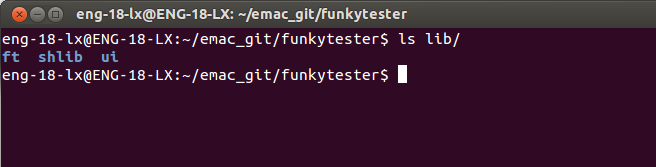
\includegraphics[keepaspectratio=true,scale=0.6]{layer_two_lib.png}}
		\captionof{figure}{Layer Two: Contents of \texttt{funkytester/lib}}
		\label{fig:lib}
	\end{minipage}
	\vspace{5pt}% gives some breathing room below

Let's look at each of these items in a little more detail:
\begin{itemize}
	\item \texttt{ft}: This is the testing code. There's a lot hidden beneath these two innocent looking letters. Don't be fooled.
	\item \texttt{shlib}: \dstar These look like shell scripts...maybe they have to do with installation?\dstar
	\item \texttt{ui}: This is the code for the user interface. You'll want to mentally steel yourself before diving into this one, as well.
\end{itemize}

Since the importance of \texttt{funkytester/bin} is mostly encapsulated by it being the location of \texttt{pytest.py}, it makes sense to now shift focus entirely to \texttt{funkytester/lib}, which is exactly what we'll do in \hyperref[sec:layer3]{\textbf{Layer Three}}.
\end{comment}

\section{Layer Three: Main Codebase}	\label{sec:layer3}
% -- Where the Shit Hits the Fan} 
%\begin{chapquote}{H. L. Mencken, \textit{Prejudices, First Series}}
%``Every normal man must be tempted, at times, to spit on his hands, hoist the black flag, and begin slitting throats."
%\end{chapquote}

% REVIEW
The main section of code falls into two groups : \texttt{ft} and \texttt{ui}. The \texttt{ft} section holds abstractions of physical items: the Unit Under Test, the testing Platform, and Platform Slots, and also the code for interactions among these abstractions. The code for the Graphical User Interface is located in the \texttt{ui} section.

\subsection{Contents of \texttt{funkytester/lib/ft}}
The directory \texttt{funkytester/lib/ft} is a package of modules. Every package must have a file called \texttt{\_\_init\_\_.py} (see \hyperref[fig:lib/ft]{\textbf{Figure \ref{fig:lib/ft}}}) so that the Python interpreter can interpret the directory as a package. Interestingly, this file can be empty. In other words, it may not do anything at all except indicate that the directory is a package. In \texttt{funkytester/lib/ft}, the \texttt{\_\_init\_\_.py} script does \textit{almost} nothing. It simply sets the \texttt{\_\_all\_\_} variable, which explicitly sets which names in the package are public. Without a defined \texttt{\_\_all\_\_} variable, all names in the package are considered public (except for those names beginning with an underscore, which is the conventional method of indicating an `internal use' object or function).

Before continuing, it is recommend to read through \hyperref[app:SQL]{\textbf{Appendix \ref{app:SQL}}} and become familiar with MySQL and sqlalchemy. \\

	\begin{minipage}{\linewidth}
		\begin{tikzpicture}
    \node [fill=codebgcolor,rounded corners=5pt]
    {{
        \begin{tabular}{l}
\begin{lstlisting}
/funkytester/lib/ft $ ls
command.py   device/   event.pyc    __init__.pyc  server/  unittest/
command.pyc  event.py  __init__.py  platform/     test/    util/
/funkytester/lib/ft $ 

\end{lstlisting}
        \end{tabular}
      }};
  		\end{tikzpicture}
		\captionof{figure}{Layer Four: Contents of \texttt{funkytester/lib/ft}}
		\label{fig:lib/ft}
	\end{minipage}
		\vspace{5pt}% gives some breathing room below

% 2DO: make the note in this paragraph a sidenote if time
There are two scripts  besides \texttt{\_\_init\_\_.py} in this directory that are not in subdirectories: \texttt{command.py} and \texttt{event.py}. \textit{Note: we'll ignore all files of the form \texttt{*.pyc} since these are just already-``byte-compiled" versions of their \texttt{.py} counterparts.} The rest of the contents of this directory are modules. How do we know? Because each of these subdirectories has its own \texttt{\_\_init\_\_.py} file. Modules, like packages, must have this file in order to indicate that the directory is a module (which just contain scripts) or a package (which contains modules and may also have scripts).

The scripts \texttt{command.py} and \texttt{event.py} are used for communicating between the platform itself (and all of its components) and the user interface.
% 2DO also, what are each of the modules? should we wait until the next section to delve into that? ****DO THIS******

\subsection{Contents of \texttt{funkytester/lib/ui}} \label{sec:ui_contents}
% 2DO
% a 'find . -name '*.php' | xargs wc -l' will show that /ft/ has 4191 LOC and /ui/
% has 1994 LOC	
Since there is both a \texttt{\_\_init\_\_.py} and a module contained in \texttt{funkytester/lib/ui}, it is a package. It's a smaller package than \texttt{ft}, but it's no less complex. In fact, since this is where the GUI is located, it could be argued that it is even more complex than the code for \texttt{ft} (user interface code is notoriously complicated).

Looking at the contents of this package -- see \hyperref[fig:lib/ui]{\textbf{Figure \ref{fig:lib/ui}}}, besides the \texttt{\_\_init\_\_.py} script (which again just sets the \texttt{\_\_all\_\_} variable), there is just one script and one module. The module is called \texttt{elements}. Within \texttt{elements} lie all of the \textit{elements} needed for a GUI programmed with GTK+ (see \hyperref[sec:GTK]{\textbf{Appendix \ref{app:GTK}}}). These elements are just more abstractions -- Python objects that represent dialogs, menus, buttons, etc. The \texttt{funct.py} script instantiates an event handler along with two different models. A model is a type of element, which will be explained in \hyperref[sec:ui]{\textbf{Chapter \ref{sec:ui}}}. For now just note that it is an abstraction needed for communication between the user interface and the event handler.\\

	\begin{minipage}{\linewidth}
		\begin{tikzpicture}
    \node [fill=codebgcolor,rounded corners=5pt]
    {{
        \begin{tabular}{l}
\begin{lstlisting}
/funkytester/lib/ft $ ls
elements/  funct.py  funct.pyc  __init__.py  __init__.pyc
/funkytester/lib/ft $ 

\end{lstlisting}
        \end{tabular}
      }};
  		\end{tikzpicture}
		\captionof{figure}{Layer Four: Contents of \texttt{funkytester/lib/ui}}
		\label{fig:lib/ui}
	\end{minipage}

%%%%%%%%%%%%%%%%%%%%%%%%%%%%%%%%%%%%%%%%%%%%%%%%%%%%%%%%%%%%%%%%%%%%%%%%%%%%%%%%%%%%%%%%%%%%%%%%%%%%%%%%%%%%%%
\chapter{The Heart of the Code: \texttt{ft}}
% 2DO
\begin{chapquote}{Xun Zi, \textit{}}
``In order to properly understand the big picture, everyone should fear becoming mentally clouded and obsessed with one small section of truth.''
\end{chapquote}

% 2DO
% platform, test are the focus; what do the other modules do (bigger pic), what 
% do command, event do (more detail than earlier section?)

\section{\texttt{platform}}
% 2DO
Before \texttt{platform} is discussed, please note \hyperref[fig:platform]{\textbf{Figure \ref{fig:platform}}}. This is a diagram of the abstractions in the \texttt{platform} directory and a way to think of their interactions. The largest abstraction in the picture is Platform and it acts as a hub for all other abstraction interactions. This Platform is the object in the code that represents the testing platform. For now, there are only two different platforms: the GE EVSC and the Quad Testset. But, as noted earlier, the code is set up so that there could be any number of testing platforms and still use the same code to set up the testing. 

In general, the names of objects (or abstractions) correspond to their respective physical counterparts. The PlatformSlot objects in the code represent slots in the physical platform. The UnitUnderTests are objects representing the boards being tested. The Product objects are a little different in that they don't represent physical objects. A Product takes information given in a manifest.yaml file that is product-specific and translates that .yaml information into Python-accessible information by means of creating a new object. This object is the Product. The reason for this is that the information provided by the manifest.yaml file is company-specific and cannot be saved in a public repository. Saving it to a .yaml file first allows any sensitive information to be protected.\\

	\begin{minipage}{\linewidth}
		\makebox[\linewidth]{
			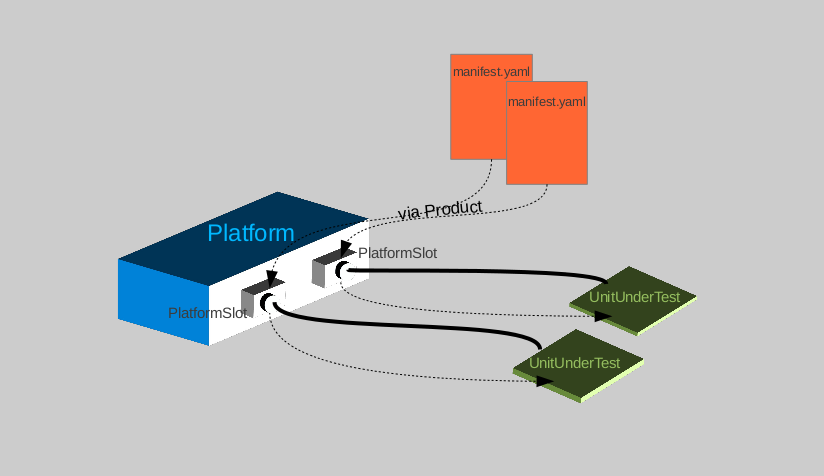
\includegraphics[keepaspectratio=true,scale=0.6]{platformslotuut0.png}}
		\captionof{figure}{Interactions among Objects in \texttt{platform}}
		\label{fig:platform}
	\end{minipage} 
	\vspace{5pt}		%give some breathing room below

Now that the basic building blocks of the \texttt{platform} module have been introduced, the process of how the control flow is passed from one object to the next as the Platform is set up will be discussed.

A good thing to keep in mind is lineage: namely, Platform is the parent of each PlatformSlot and each PlatformSlot has a single UnitUnderTest child. Note that for each set up, we will deal with only one Platform. In the figure above, the parent-to-child lineage shows up as physical attachments among the objects. In this diagram, the Platform has two PlatformSlots attached to it, each of which are attached to a UnitUnderTest (by the black cords). The dotted lines with arrows show a `weaker' attachment. These arrows represent a flow of information from the manifest.yaml files to a Product object to a PlatformSlot to the UnitUnderTest. Each UnitUnderTest will have its own manifest.yaml file since each represents a single product. 

%REVAMP
For example, one UnitUnderTest may be a G4 while the other is a G2. Since the GE EVSC has only one PlatformSlot, the picture above would not be possible (it would only have one PlatformSlot), but it gives a good intuition for what's going on. The Quad Testset would have four PlatformSlots.

%REVAMP -- Product was already covered. i like this explanation better, though.
A note about the Product, which is a Python object, but doesn't have a picture (just a small mention) in the diagram. This is because there isn't a physical analogue to the Product object. The Product is just a means of gathering information from a manifest.yaml file and making it Python-accessable. %more

%transition
PlatformSlot accesses both UnitUnderTest and Product and gives the UnitUnderTest pertinent information from Product.

\section{\texttt{test}}
% REVIEW
There are two different abstractions within the \texttt{test} module: tests and actions. Each test that the user wishes to run on the Unit Under Test must have its details set up in a specification file. The specification for a test holds the recipe for running the test: a set of actions. For example, one test might test a UUT's ability to read from a file. That test must mount, try to read, and then unmount. Each of these three things is an action. A read test simply runs these three actions in order.

%fix the output here for funkytester/resources/products/<platform>/spec
The specification files are actually written as .yaml files and are saved in the directory with the path \texttt{funkytester/resources/products/<platform>/spec} on the testset. Each board to be tested has its own specification file for the tests to be run on it. Then  \texttt{specification.py} translates the test specs from the .yaml file into Python objects so we can access the specifications in \texttt{action.py}.

To review, the specification file gives specifics for each test ``recipe": a list of actions that must be called in order to run the test. The \texttt{test.py} script gives us an abstraction of each test, which can be used to access the action object created by \texttt{action.py}. Test objects can then later be accessed by other parts of the code.\\

	\begin{minipage}{\linewidth}
		\makebox[\linewidth]{
			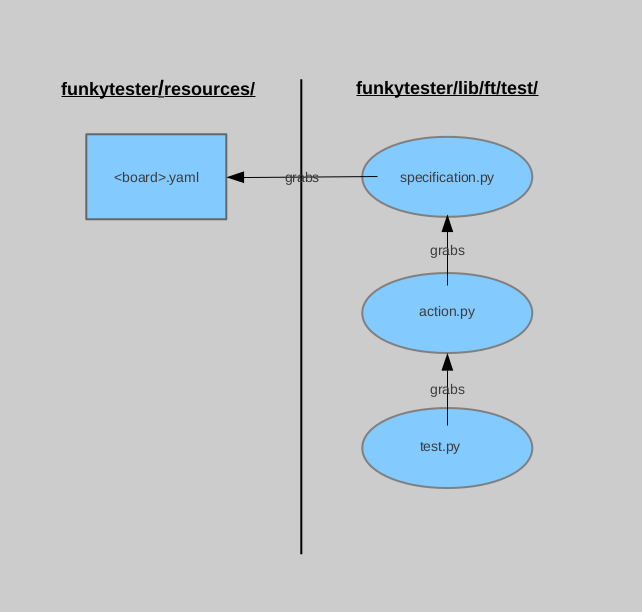
\includegraphics[keepaspectratio=true,scale=0.6]{FT_test.png}}
		\captionof{figure}{Interactions among Objects in \texttt{test}}
		\label{fig:test}
	\end{minipage}
	\vspace{5pt}		%give some breathing room below

\section{Communicating With the User Interface}
% events and commands
Events are messages from the platform to the user interface, whereas commands are messages that are sent from the user interface to the platform. Both routes of communication are needed in order to have a properly working interface. Each side (the front-end UI and the back-end platform) must have feedback from the other in order to respond appropriately and give the user an idea of what is happening. For instance, if a test fails, the user should be notified and if possible, given a short message as to why the failure occurred.\\

%communication breakdown
	\begin{minipage}{\linewidth}
		\makebox[\linewidth]{
			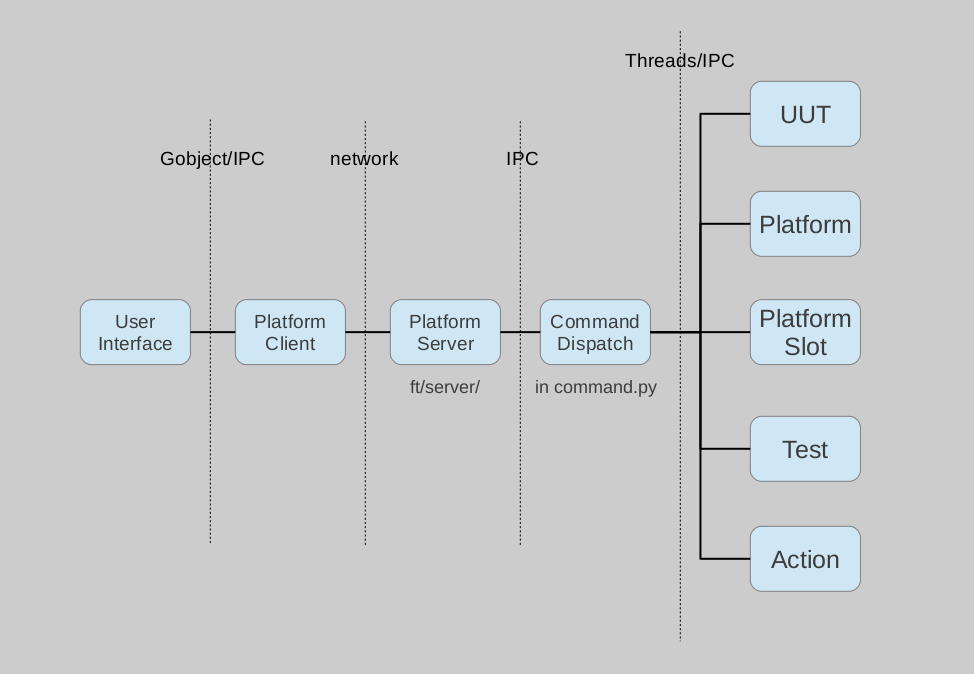
\includegraphics[keepaspectratio=true,scale=0.6]{comm.png}}
		\captionof{figure}{Communication Among Objects in \texttt{ui/} and \texttt{ft/}}
		\label{fig:ft_comm}
	\end{minipage} 
	\vspace{5pt}		%give some breathing room below

%%%%%%%%%%%%%%%%%%%%%%%%%%%%%%%%%%%%%%%%%%%%%%%%%%%%%%%%%%%%%%%%%%%%%%%%%%%%%%%%%%%%%%%%%%%%%%%%%%%%%%%%%%%%%%
\chapter{The User Interface Code: \texttt{ui}} \label{sec:ui}
% 2DO
\begin{chapquote}{Linus Torvalds \textit{}}
``In many cases, the user interface to a program is the most important part for a commercial company: whether the programs works correctly or not seems to be secondary."
\end{chapquote}
%say stuff about PyGTK -- hlink to appendix
%2DO
When looking into the GUI code, please note that the flow is completely different from the back end code. The GUI is based on an event-driven programming paradigm, which is quite different than the other code in the FunkyTester. For more information about event-driven programming and the GTK GUI, please refer to \hyperref[app:GTK]{\textbf{Appendix \ref{app:GTK}}}.

It was mentioned in \hyperref[sec:ui_contents]{\textbf{Section \ref{sec:ui_contents}}} that \texttt{funkytester/lib/ui} contains one module and one script (besides the obligatory \texttt{\_\_init\_\_.py}). The module \texttt{elements} and its contents will now be looked at with greater scrutiny.

% talk about /elements/
\section{\texttt{elements}}
In the following subsections, the modules within \texttt{elements} will be explored, for now just focus on the scripts in this directory, ignoring \texttt{\_\_init\_\_.py}.\\

%2DO: where we puttin this?
	\begin{minipage}{\linewidth}
		\begin{tikzpicture}
    \node [fill=codebgcolor,rounded corners=5pt]
    {{
        \begin{tabular}{l}
\begin{lstlisting}
/funkytester/lib/ui/elements $ ls
adapters/       functeventhandler.py   generic.py    menus/    utils.pyc
dialogs/        functeventhandler.pyc  generic.pyc   models/
functester.py   functwidgets.py        __init__.py   pages/
functester.pyc  functwidgets.pyc       __init__.pyc  utils.py
/funkytester/lib/ui/elements $ 
\end{lstlisting}
        \end{tabular}
      }};
  		\end{tikzpicture}
		\captionof{figure}{Contents of \texttt{funkytester/lib/ui/elements}}
		\label{fig:ui/elements}
	\end{minipage}
		\vspace{5pt}% gives some breathing room below
		
%itemize the scripts: say what each does: functester, functhandler, functwidgets, generic, utils
\begin{itemize}
	\item \texttt{functester.py}: Sets up the Funky Tester window in the GUI and sets in motion the construction of the menus, pages, and dialogs. Also connects event handlers to events (via the connect function) and holds callbacks for each type of event. %all of this correct?
	\item \texttt{functeventhandler.py}: queues events that are emitted from the platform and handles each in turn. Each event is handled based on the type of event it is (for example: a Test event or a Platform event).
	\item \texttt{functwidget.py}: Two classes: PlatformSlotSetupWidget, which inherits from gtk.Frame; and AbstractSelectionWidget, which inherits from gtk.VBox. An AbstractSelectionWidget sets up a selection box, determines when a selection has been made, and passes the flow of control appropriately (via callback functions).
	\item \texttt{generic.py}: Again, two classes: FunctTreeStore, which is a gtk.TreeStore object that is used for storing adapters; and the GenericAdapter class, which inherits from gobject.GObject and is the parent for the adapters (to be introduced shortly).
	\item \texttt{utils.py}: A single class for creating a labeled hbox. Miscellaneous, but very important functionality.
\end{itemize}

% 2DO a different order might make more sense for the following sections
%not sure if i want these grouped together in an itemized list or if i want 
% separate subsections for each...
\subsection{Modules in \texttt{elements}}

\begin{itemize}
	\item\texttt{adapters}: Adapters maintain the state of platform objects; that is, the state of the Platform, PlatformSlots, Tests, Actions, and UnitUnderTests.
	\item\texttt{models}: A TreeView object is essentially a group of descriptors that are used to describe columns. The TreeView object is then populated with models, which are rows, each of which have column attributes from the TreeView object. For example: TreeView attributes across the top of a chart (x-axis) and models as the label down the side (y-axis).\\
	Testmodels consist of rows of units (UUTs) and two layers of nested rows: tests and actions. Each of these layers of the testmodel have associated menus (see below).
	\item\texttt{pages}: Pages are the containers for TreeView-model objects. They are seen in the GUI as the tabs labeled ``Slot Setup" and ``Test Manager".
	\item\texttt{dialogs}: Dialogs are any pop-up windows. They may ask for information from the user (eg: select a product or version), or they may just give the user information. This is the case with warnings that pop up with traceback information in the case of an error.
	\item\texttt{menus}: These are content menus. At the moment, they are seen only as the menus that pop up when an item in the GUI is right-clicked. There are four different kinds of menus: slot menus, which are associated with the slot models; and UUT, test, and action menus, which are associated with a test model.
\end{itemize}

Now that some of the details in the user interface code have been looked at, the highest level of the \texttt{ui} architecture needs to be re-examined. %now talk about what funct is doing --> how the flow goes (where it pulls info from) -- a general overview
\section{Overview of \texttt{funct}}
In this section the top level of the user interface, \texttt{funct}, will be explored. There exists only one function in \texttt{funct.py}, that function is \texttt{main}. This is where the initial models and event handlers are called to start building the GUI. Also, \texttt{funct} is where the main GTK loop is started. This loop is responsible for responding to user inputs and displaying the proper output. 
\newpage

%%%%%%%%%%%%%%%%%%%%%%%%%%%%%%%%%%%%%%%%%%%%%%%%%%%%%%%%%%%%%%%%%%%%%%%%%%%%%%%%%%%%%%%%%%%%%%%%%%%%%%%%%%%%%%
\section*{Quotes}
%just needed a place to hold these quotes because I like them and I want to use 
% them at some point in this document if possible
\begin{chapquote}{Ken Thompson \textit{}}
``You can’t trust code that you did not totally create yourself."
\end{chapquote}

\begin{chapquote}{Christer Ericson \textit{}}
``Premature abstraction is like ebola; it makes my eyes bleed.''
\end{chapquote}

\begin{chapquote}{Sheldon Cooper, \textit{The Big Bang Theory}}
``You're right. I should embrace the chaos.''
\end{chapquote}

\begin{chapquote}{C.A.R. Hoare, \textit{The 1980 ACM Turing Award Lecture}}
``There are two ways of constructing a software design: One way is to make it so simple that there are obviously no deficiencies and the other way is to make it so complicated that there are no obvious deficiencies.''
\end{chapquote}

\begin{chapquote}{Charles M. Strauss \textit{}}
``Mostly, when you see programmers, they aren’t doing anything. One of the attractive things about programmers is that you cannot tell whether or not they are working simply by looking at them. Very often they're sitting there seemingly drinking coffee and gossiping, or just staring into space. What the programmer is trying to do is get a handle on all the individual and unrelated ideas that are scampering around in his head."
\end{chapquote}

\begin{chapquote}{Douglas Adams}
``A common mistake that people make when trying to design something completely foolproof is to underestimate the ingenuity of complete fools.''
\end{chapquote}
%%%%%%%%%%%%%%%%%%%%%%%%%%%%%%%%%%%%%%%%%%%%%%%%%%%%%%%%%%%%%%%%%%%%%%%%%%%%%%%%%%%%%%%%%%%%%%%%%%%%%%%%%%%%%%
\section*{}

%-------------------------------------------------------------------%
\begin{appendices}
%---------------------------------------%
\chapter{Commands to Remember} \label{app:cmd}

\section{Cloning the Git Repositories} \label{sec:gitcloning}
Begin at the place all good projects begin: by opening a terminal. Navigate to the directory you want to keep the code directory (which will be named \texttt{funkytester}). Then type:\\

  \begin{tikzpicture}
    \node [fill=codebgcolor,rounded corners=5pt]
    {{
        \begin{tabular}{l}
\begin{lstlisting}
$ git clone --recursive git@git.emacinc.com:public/suites/funkytester.git
$ cd funkytester
$ git clone --recursive git@git.emacinc.com:private/ft/resources.git ext/emac 
$
\end{lstlisting}
        \end{tabular}
      }};
  \end{tikzpicture}


\section{Logging into the Testset Machine via SSH} \label{sec:SSH}
From any directory on your local mahcine, you can run the following command to SSH into the testset machine:\\

  \begin{tikzpicture}
    \node [fill=slorange,rounded corners=5pt]
    {{
        \begin{tabular}{l}
\begin{lstlisting}
$ ssh -X test@10.0.2.152
test@10.0.2.152's password: test
<<copyright and last log-in info>>
$
\end{lstlisting}
        \end{tabular}
      }};
  \end{tikzpicture}


\section{Running the Testset Software} \label{sec:run}
The default method for running the testset software is now through a server socket implementation, meaning we need a server and a client to run it. On your local machine, you'll want to open two terminals. In the first, we'll SSH into the testset machine and run the server side. In the second, we'll run the client side. In the first terminal, type:\\

 \begin{tikzpicture}
 	   \node [fill=slorange,rounded corners=5pt]
    		{{
        		\begin{tabular}{l}
	\begin{lstlisting}
$ ssh -X test@10.0.2.152
test@10.0.2.152's password: test
<<copyright and last log-in info>>
$ cd projects/funkytester-test
$ ./bin/pytest.py --server-only -a ext/emac/manifest.yaml -H 10.0.2.152 -p 9999
server address: 10.0.2.152, server port: 9999
$
	\end{lstlisting}
    		    \end{tabular}
	      }};
  \end{tikzpicture}
  	
The testset machine is now waiting for a client to talk to. We can have our local machine play that role by typing the following into the second terminal:\\

 \begin{tikzpicture}
 	   \node [fill=slgreen,rounded corners=5pt]
    		{{
        		\begin{tabular}{l}
	\begin{lstlisting}
$ ./bin/pytest.py --client-only -a ext/emac/manifest.yaml -H 10.0.2.152 -p 9999
$ 
	\end{lstlisting}
    		    \end{tabular}
	      }};
  \end{tikzpicture}

If the testset software still doesn't run, you may have to update your local machine's submodules. To do this, type:\\

 \begin{tikzpicture}
 	   \node [fill=slgreen,rounded corners=5pt]
    		{{
        		\begin{tabular}{l}
	\begin{lstlisting}
$ git submodule update --merge
$ 
	\end{lstlisting}
    		    \end{tabular}
	      }};
  \end{tikzpicture}

Then try running the software again. To exit out of the server, press CTL+z to background the task, then to terminate it, type:\\

 \begin{tikzpicture}
 	   \node [fill=slblue,rounded corners=5pt]
    		{{
        		\begin{tabular}{l}
	\begin{lstlisting}
$ kill %1
$ 
	\end{lstlisting}
    		    \end{tabular}
	      }};
  \end{tikzpicture}

{\ww Something to watch out for is that some error conditions can lead to the server
shutting down without properly letting go of the port to which its socket is
bound. If this happens, next time you try to start the server you will get an
address already in-use error message in which case you can simply use a
different port number ('-p 9998' for example). You will need to use that new
port number on both the server and the client invocation.}

\begin{comment} % The following is now deprecated. The default method for running
	% the testset software is now via the server socket implementation.
	On the Testset machine:\\

  	\begin{tikzpicture}
 	   \node [fill=slblue,rounded corners=5pt]
    		{{
        		\begin{tabular}{l}
	\begin{lstlisting}
	$ cd projects/funkytester
	$ ./bin/pytest.py -p ext/emac/manifest.yaml
	\end{lstlisting}
    		    \end{tabular}
	      }};
  	\end{tikzpicture}


	On your local machine, navigate to the \texttt{funkytester} directory, then 	
	type:\\

	  \begin{tikzpicture}
    		\node [fill=slgreen,rounded corners=5pt]
    		{{
        		\begin{tabular}{l}
	\begin{lstlisting}
	$ ./bin/pytest.py -p ext/emac/manifest.yaml
	$
	\end{lstlisting}
    		    \end{tabular}
      	}};
  	\end{tikzpicture}
\end{comment}

\subsection{Troubleshooting} \label{sec:trouble}
%REVIEW
%itemize these
Make sure you have all necessary software installed on your machine. Check the \texttt{INSTALL} file in the main \texttt{funkytester} directory.

Try updating submodules (from \texttt{funkytester} directory):\\

	  \begin{tikzpicture}
    		\node [fill=slgreen,rounded corners=5pt]
    		{{
        		\begin{tabular}{l}
	\begin{lstlisting}
$ git submodule update --merge
$
	\end{lstlisting}
    		    \end{tabular}
      	}};
  	\end{tikzpicture}
  	
There may be issues with old byte-compiled files, so remove these from your local machine. From the \texttt{funkytester} directory:\\

	  \begin{tikzpicture}
    		\node [fill=slgreen,rounded corners=5pt]
    		{{
        		\begin{tabular}{l}
	\begin{lstlisting}
$ rm -rf 'find -iname "*.pyc"'
$
	\end{lstlisting}
    		    \end{tabular}
      	}};
  	\end{tikzpicture}

\section{Creating a Remote Mount Point} \label{sec:fsmount}
First, make sure you have sshfs installed. Then go to the parent directory of \texttt{funkytester} and create a remote file system mount point (as far as I know, this is just a directory that we use as mount point):\\
%2DO

  \begin{tikzpicture}
    \node [fill=slgreen,rounded corners=5pt]
    {{
        \begin{tabular}{l}
\begin{lstlisting}
$ mkdir funkytester-remote
$
\end{lstlisting}
        \end{tabular}
      }};
  \end{tikzpicture}

Now that you have a mount point, you can navigate to its parent directory and mount the testset machine's filesystem to \texttt{funkytester-remote} by typing:\\
%2DO

  \begin{tikzpicture}
    \node [fill=slgreen,rounded corners=5pt]
    {{
        \begin{tabular}{l}
\begin{lstlisting}
$ sshfs test@10.0.2.152:projects/montana/funkytester funkytester-remote
$
\end{lstlisting}
        \end{tabular}
      }};
  \end{tikzpicture}

The purpose of making a mount point like this on your local machine is to make changing things in the code and testing it on the testset machine easier for you. Basically, you have access to any tools you always have on your machine (for example -- your favorite text editor), but the changes you make to the code do actually get transferred to the testset machine. If you then, in say another terminal, SSH into the testset machine and navigate to \texttt{projects/montana/funkytester}, you can run the code with your changes without interfering with Wayne's code (which is in \texttt{projects/funkytester}, remember? The code in \texttt{projects/montana/funkytester} is a different copy of the code -- a copy that we are allowed to play around with.)

%---------------------------------------%
\chapter{Python} \label{app:python}
% organize cheat sheet .pdfs better -- separate place for them? or just retype?
\includepdf[pages={1},scale=.8,pagecommand=\section{Useful Python Odds 'n Ends}]{python_cheat_sheet.pdf}
\includepdf[pages={2-3},scale=.8]{python_cheat_sheet.pdf}
\includepdf[pages={1},scale=.8,pagecommand=\section{Python Quick Reference}]{python_quick.pdf}

%---------------------------------------%
\chapter{PyGTK and the Basics of a Graphical User Interface} \label{app:GTK}
% REVAMP
\begin{chapquote}{Hal Sparks \textit{}}
``\ldots there's no calculator for human interaction.''
\end{chapquote}

% i'm not sure if i want to include this or not. it's a nice, friendly little 
% description of a GUI, highlighting the important parts.
\begin{comment}
% maybe put this in a box on the side of the page or something
\textbf{What is a GUI?}
mathworks.com says...
\href{http://www.mathworks.com/help/matlab/creating_guis/what-is-a-gui.html}{source}

	\begin{quotation}
	A graphical user interface (GUI) is a graphical display in one or more windows 
	containing controls, called components, that enable a user to perform 
	interactive tasks. The user of the GUI does not have to create a script or type 
	commands at the command line to accomplish the tasks. Unlike coding programs to 
	accomplish tasks, the user of a GUI need not understand the details of how the 
	tasks are performed. GUI components can include menus, toolbars, push buttons, 
	radio buttons, list boxes, and sliders—just to name a few.
	\end{quotation}

\end{comment}
PyGTK is what allows us to create a \textbf{G}raphical \textbf{U}ser \textbf{I}nterface. This part of the code is the GUI -- a notoriously difficult programming task. It's my understanding that all GUIs are programmed under the \textit{event-driven programming} paradigm. This Appendix is not intended to introduce or teach this paradigm, but interested parties can find a fantastic paper online: \href{http://eventdrivenpgm.sourceforge.net/}{\textbf{Stephen Ferg's \textit{Event-Driven Programming}}}.

But let's think about what a GUI does for a minute. It displays some information to the user, waits for the user to press a button or scroll or exit or in some way interact with the interface, and then if all goes well, the interface will react in some useful, logical (or at least intuitive) way. 

That is a lot. 

I mean, it's a lot for a human to interact successfully with other humans, and we tend to be much more adaptable than machines. Since (at least at this point in history) machines need to be told explicitly what to do, there must be some systematic way for the machine to handle user interactions. And there is. In fact, the things that handle user interactions are appropriately called handlers. The handler waits for some previously determined signal, then calls some other function when it finds its signal. The `other function' that is called by the handler has a name, too: a callback function.
%explain what GTK+ is, briefly. like, hardly even explain it.
\section{Events, Signal Handlers, \& Callback Functions}
% 2DO
There were a couple of ideas and terms I threw at you in the last section that need some hashing out. For our purposes, signals and events can be thought of as the same thing. Basically, some event happens that triggers a signal to be fired. That signal is then caught by some function whose sole purpose is to catch one specific type of signal and then call another function in response. This response function is the callback function.

Catching a signal is a phrase that is thrown around a lot without much explanation. It may seem a bit convoluted at first, but it's actually based on a very simple idea. Here's an example:
% 2DO


% figure out which way you'd like to have the code represented. neither is ideal at this point.

\begin{center}
  \begin{tikzpicture}
    \node [fill=codebgcolor,rounded corners=5pt]
    {{
        \begin{tabular}{l}
\begin{lstlisting}
class Buttons
	
	# callback functions are defined outside of the constructor
	def callback(self, widget, data):
    		print "Hello, %s was pressed" % data

	# the constructor
	def __init__(self):
		# create a dialog window
		self.window = gtk.Window(gtk.WINDOW_TOPLEVEL)
			
		# create a button called "Button 1"
		self.button1 = gtk.Button("Button 1")
			
		# create a second button called "Button 2"
		self.button2 = gtk.Button("Button 2")
			
		# if button1 is clicked, then we will call callback(),
		# passing "button 1" to it (ie: "button 1" becomes 
		# callback()'s data)
		self.button1.connect("clicked", self.callback, "button 1")
			
		# similarly for button2
		self.button2.connect("clicked", self.callback, "button 2")
\end{lstlisting}
        \end{tabular}
      }};
  \end{tikzpicture}
\end{center}

This is not a full program, so don't try to run it. I've left out essential pieces that make the dialog box and buttons appear (and other useful things like being able to exit this program) so that we can look just at the callback function, the signals, and the signal handlers. 

Identifying the callback function is easy enough -- its name is callback and the comments denote it as the callback function, too. The only signal we deal with is ``clicked" which is emitted internally (that is, we don't have to worry about how it appears -- GTK+ does this for us). To elaborate, we don't have to be able to detect when a user clicks a button on the GUI; we just need to know that a signal is emitted that we need to catch.

So where are the signal handlers? There are exactly two. The first is \texttt{self.button1.connect()} and the second is \texttt{self.button2.connect()}. Both are waiting for the same signal, but each is associated to a different button. So when \texttt{button1} is clicked, \texttt{self.button1.connect()} gets called. And this handler exists solely to pass the flow of activity to \texttt{callback()}. The last argument (and any subsequent arguments), ``button 1", is the argument that gets passed into \texttt{callback()}.

% what Stephen Ferg has to say: ``The job of the dispatcher is to take each event
% that comes to it, analyze the event to determine its event type, and then send
% each event to a handler that can handle events of that type." (pg. 11)

\section{From GTK+ to PyGTK}
There are two levels of abstraction we are interested in for GUI programming as it relates to the FunkyTester code. The more abstract of the two levels is GTK+, which provides a means for interacting with the user. It detects when parts of the GUI are clicked, resized, moved, dragged, or what have you by the user. When programming with PyGTK, we don't need to know how those details are handled. We just need to know what the signals each of these events emits are called so that we can appropriately handle them in our Python code. 

Think of GTK+ as the liaison between the user and our code. Let's follow the flow of communication. Say the user clicks some Button A. GTK+ then detects this click and emits a ``clicked" signal for any interested parties to pick up. If there is a signal handler in place for ``clicked", then that handler will be called. If no signal handler has been written for ``clicked", then nothing happens. For the sake of simplicity, let's assume a signal handler exists for this signal. Then that handler calls some other function which will carry out the task the user expects to be performed when pressing Button A. When finished, the task emits some ``I'm finished" signal which gets passed to GTK+ and subsequently to the user. In this way, the user always gets feedback to know if the task was completed. 

To communicate with our Python code, though, GTK+ needs its own liaison. This liaison is PyGTK. We use PyGTK objects and functions to translate between Python and GTK+. The reason for this is so that developers using other languages besides Python can use GTK+ to create GUIs as well. (Incidentally, that's why we have the PyGTK level of abstraction in the first place.) We say GTK+ is a library of functions that creates a user interface and that PyGTK is a library of Python wrapper functions for GTK+.

%---------------------------------------%
\chapter{SQLAlchemy: The Least You Need to Know}	\label{app:SQL}
\begin{chapquote}{Carlos Bustamante; Molecular Biologist, UC Berkeley \textit{}}
``Being a scientist means living on the borderline between your competence and your incompetence. If you always feel competent, you aren't doing your job."
\end{chapquote}

To get to the point of this section, a we'll need few preliminary explanations (along with a slew of acronyms). Namely, we should first talk about \textbf{RDBMS}s, \textbf{SQL}, \textbf{ORM}s, and by the time those items are explained, \textbf{SQLAlchemy} will be a piece of cake. After all of that, we can look into how and why the FunkyTester code uses SQLAlchemy.
	\begin{itemize}
	\item\textbf{RDBMS}: RDBMS stands for \textbf{R}elational \textbf{D}atabase \textbf{M}anagement \textbf{S}ystem. It does what it sounds like it does: manages databases. And it does this based on a relational model, which means that data is presented to the user as a collection of tables that each consist of columns and rows. You can think of each column as representing some characteristic (like color, size, age, viscosity, or whatever other kind of adjective you'd like to give an item) and each row as representing an object that has all those column characteristics. Here are some examples of RDBMSs: Oracle Database, Microsoft SQL Server, MySQL, PostgreSQL, and SQLite. It would probably be nice to know at this point what SQL is.
	\item\textbf{SQL}: SQL is an acronym for \textbf{S}tructured \textbf{Q}uery \textbf{L}anguage. So it's just a language, and it was designed for communicating with a database. It's the layer of abstraction hovering right above the RDBMS. Pretty simple.
	Now, the ``Query" part of SQL comes from the idea that if the database is large enough (which, of course it will be -- why else would we use so much abstraction?;)), it's going to be difficult to find particular elements or groups of elements in the database by hand, so we'll want to query the database for the elements we seek. For a basic overview, watch this \href{http://www.youtube.com/watch?v=EUB113i_mzA}{\textbf{SQL introduction}}.
	\item\textbf{ORM}: Ah, the \textbf{O}bject \textbf{R}elational \textbf{M}apper. Let's segue once more and talk a little about object-oriented programming and databases. Object-oriented programming languages like Python use objects to potentially hold a gosh-ton of information and plenty of layers of abstractions\ldots These objects can get kind of messy. Ideally, we'd be able to represent objects in our code as elements in our database -- for easy storage, easy access, etc. But because objects in our code can become so complex, it's not so simple to put them into a table-friendly format. That's why we have ORMs -- they act as translators between our Python code's objects and the elements of the database we are using.\\
	An ORM can take a Python object, make its attributes into column characteristics and call it a row in a table. It can also go the other way -- take an element from the table and create a Python object. Essentially, it makes our lives easier because we can manipulate Python objects as though they were in the database and not have to think about the complications involved.\\
	Let's recap now, to emphasize the difference between SQL and ORMs. An ORM will translate Python objects into elements that can be put into a table in our database. Whereas SQL is a language that accesses that database once it has been created.
	\item\textbf{SQLAlchemy}: At long last, we get to our initial \textit{objet de d\'esir}: SQLAlchemy. I promised this part would be easy, and it is. SQLAlchemy is just an ORM. It's the ORM that is used in the FunkyTester code and that's that.  For understanding the FunkyTester code, it's not really essential to understand how this is done, but if you are interested, \href{http://docs.sqlalchemy.org/en/rel_0_5/ormtutorial.html}{\textbf{here}} is a link to a tutorial. It may be helpful to quickly run through just so that you are able to recognize SQLAlchemy portions of FunkyTester code.
	\end{itemize}

Before we get too carried away, let's reign it back in to the FunkyTester code. One of the goals of the testset is to keep a record of tests and the results of those tests so that it's possible to check records if something goes awry. This is done by logging certain testing data into a database. For EMAC, we're using Achievo. That's about the extent of my knowledge on the subject, but I do think that there will be more work done to implement this idea in the near future.

%---------------------------------------%
\chapter{Git}	\label{app:git}
If you haven't had much experience with Git, you'll definitely want to spend a little time going through a tutorial. There are plenty available, so just type ``git tutorial" into your favorite search engine and go forth. Once you have the basics down, watch this video for an explanation of Git concepts using Tinker Toys: \href{http://blip.tv/open-source-developers-conference/git-for-ages-4-and-up-4460524}{\textbf{Git for Ages 4 and Up}}.\\
In addition to the ``git cheat sheet" attached below, there are a few other git commands that I have found useful:
	\begin{itemize}
	\item clone the remote repository recursively: \texttt{git clone --recursive git@git.emacinc.com:<path>.git}
	\item rename a local branch: \texttt{git branch -m <oldname> <newname>}
	\item delete a remote branch reference: \texttt{git branch -d -r origin/<nameofbranchtodelete>}
	\item push to a remote branch: \texttt{git push origin <nameofbranchtopush>:<destinationbranchname>}
	\item list all branches: \texttt{git branch -a}
	\item list remote branches only: \texttt{git branch -r}
	\item get the working tree status of a repository (that is, see what has been changed and see what is in the index/staging area): \texttt{git status}
	\item give a list of directories you have read/write permissions for: \texttt{ssh git@git.emacinc.com info}
	\item Note that in Git, the term ``ref" is a general name encompassing \textbf{branches, tags,} and \textbf{SHA256} (the commit ID).
	\end{itemize}
\includepdf[pages={1},scale=.8]{git_cheat_sheet.pdf}

%---------------------------------------%
\chapter{Worth a Mention} \label{app:last}
\section{Make} \label{app:make}
%REVIEW
Since I don't know much about make myself, I'll leave you with a few quotes and a tutorial to get you started. I will stress that you do not need to be familiar with make in order to understand the FunkyTester code, though.

\begin{quote}
``Make is the oldest and best known build tool, a utility that allows a programmer to build or rebuild source code files into a new version of a program."
\end{quote}
\hfill -- \href{http://whatis.techtarget.com/definition/make}{\textbf{techtarget.com}}

\begin{quote}
``The make utility is a software engineering tool for managing and maintaining computer programs. Make provides most help when the program consists of many component files. As the number of files in the program increases so to does the compile time, complexity of compilation command and the likelihood of human error when entering command lines, i.e. typos and missing file names."
\end{quote}
\hfill --\href{http://capone.mtsu.edu/csdept/FacilitiesAndResources/make.htm#What%20make}
{\textbf{mtsu.edu}}

And the tutorial I promised: \href{http://mrbook.org/tutorials/make/}{\textbf{mrbook.org/tutorials/make/}}
\newpage

\section{Doxygen} \label{app:doxy}
%REVIEW
Doxygen is a documentation generator. It takes code as an argument and when run, generates documentation based on the comments in the code. If that style of commenting is used throughout the code, it makes documentation as easy as running a command in the command line, instead of having to go through everything each time. It can be configured to output a number of files, including \LaTeX\hspace*{.25pt} and html.

In order for the documentation to be generated correctly, the code must have comments written in a particular fashion. Doxygen then generates diagrams and descriptions of the code that can be reviewed by other developers.

% code snippet of 
% http://www.stack.nl/~dimitri/doxygen/manual/docblocks.html#pythonblocks
% plus the particular style wayne wanted

This is the commenting style we use in the code:\\

\begin{center}
  \begin{tikzpicture}
    \node [fill=codebgcolor,rounded corners=5pt]
    {{
        \begin{tabular}{l}
\begin{lstlisting}
## @package pyexample
# Documentation for this module.
# 
# More details.
#
def funct():
	pass
	
## Documentation for a class.
#
# More details.
#
class PyClass:

	##  The constructor.
	#
	def __init__(self):
		self.memVar = 0;
					
	## Documentation for a method.
	#
	# @param self The object pointer.
	#
	def PyMethod(self):
		pass
		
	## A class variable.
	#
	classvar = 0;
\end{lstlisting}
        \end{tabular}
      }};
  \end{tikzpicture}
\end{center}

\end{appendices}

\end{document}
